\section{The Potential of the Charge, Dielectric, and Disc Problem}
\subsection{The Complex Potential of the Disc}
\hspace{0em}\indent For a typical complex potential, it is free to use either the real or imaginary part to be the voltage. However, we will set the imaginary part as the voltage, because we require $r=1$ to be an equipotential, $\Im \left[w(|\zeta|=1)\right]=0$ , by adding $\overline{w}(\zeta^{-1})$. The complex potential of the charge is\vspace{-1.em}
\[
w_0(\zeta)=\im \log (\zeta-\zeta_0)\vspace{-1.5em}
\]
and adding
\[
\overline{w_0}(\frac{1}{\zeta}) = -\im \log (\frac{1}{\zeta}-\Bar{\zeta_0})
\]
This generates two physical entities: a sink $-\im\log (1-\zeta\zeta_0)$ at $1/\overline{\zeta_0}$ , and a source $\im\log(\zeta)$ at $\zeta = 0$ . For a point charge at \(\zeta_\alpha\) and for the unit circle to be an equipotential, two extra charges of opposite sign must be added.

\subsection{The Induced Charges of the Dielectric}
% The effect of the charges in the dielectric is investigated using conformal mapping and yields surprising results that may help understand the properties of this geometric form of a dielectric.
\hspace{0em}\indent 
The disc induces two charges inside, which may affect the dielectric and therefore require investigation. The charge at \(\zeta = 0\) does not influence the dielectric except on the arc, as proved in section (\ref{cpt:charged disc}). However, the charge at \(1/\overline{\zeta_\alpha}\) may induce surface charge in the dielectric. 

Suppose the charge in the disc off the origin induces a charge in the dielectric; it will induce two more charges inside the disc, the twice-induced charges. As this process continues, the voltage will evolve into a series\vspace{-0.5em}
\[
q\log (\zeta-\zeta_{\alpha})+\frac{q}{\epsilon}\log (\zeta-\zeta_1)+\frac{q}{\epsilon^2}\log (\zeta-\zeta_2)+...\vspace{-0.5em}
\]

The dielectric is not flat, and we are uncertain about the possibly induced charge. To determine the possible induced charge, map the surface of the dielectric to a flat one, with
\[\zeta=z-\sqrt{z^2-1}\]
\begin{figure}[H]
    \centering
    \adjustbox{frame=0.25pt,frame,margin=0.15,color=mycolor}{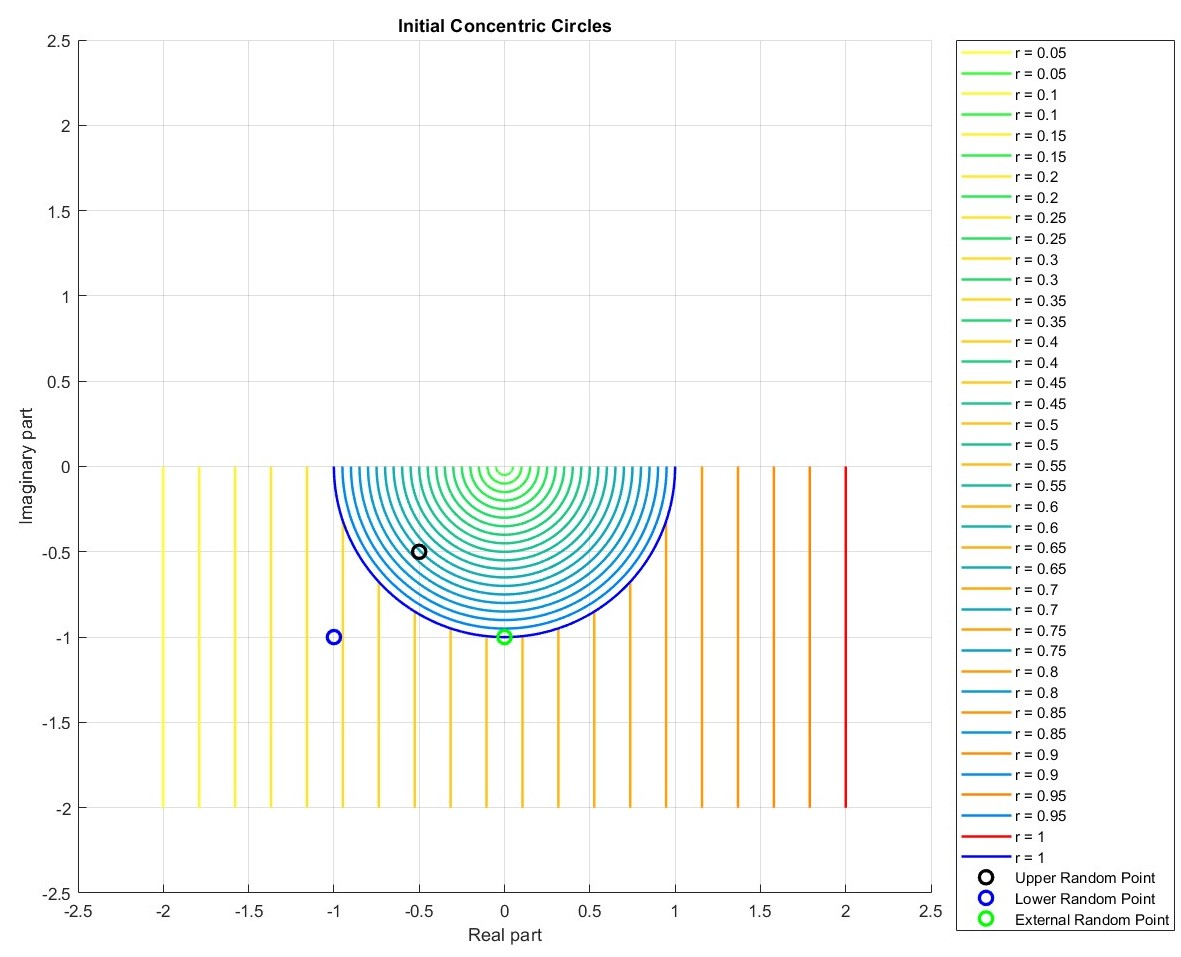
\includegraphics[width=0.493\linewidth]{Figs/semi circle and dieletric}}\hfill
    \adjustbox{frame=0.25pt,frame,margin=0.15,color=mycolor}{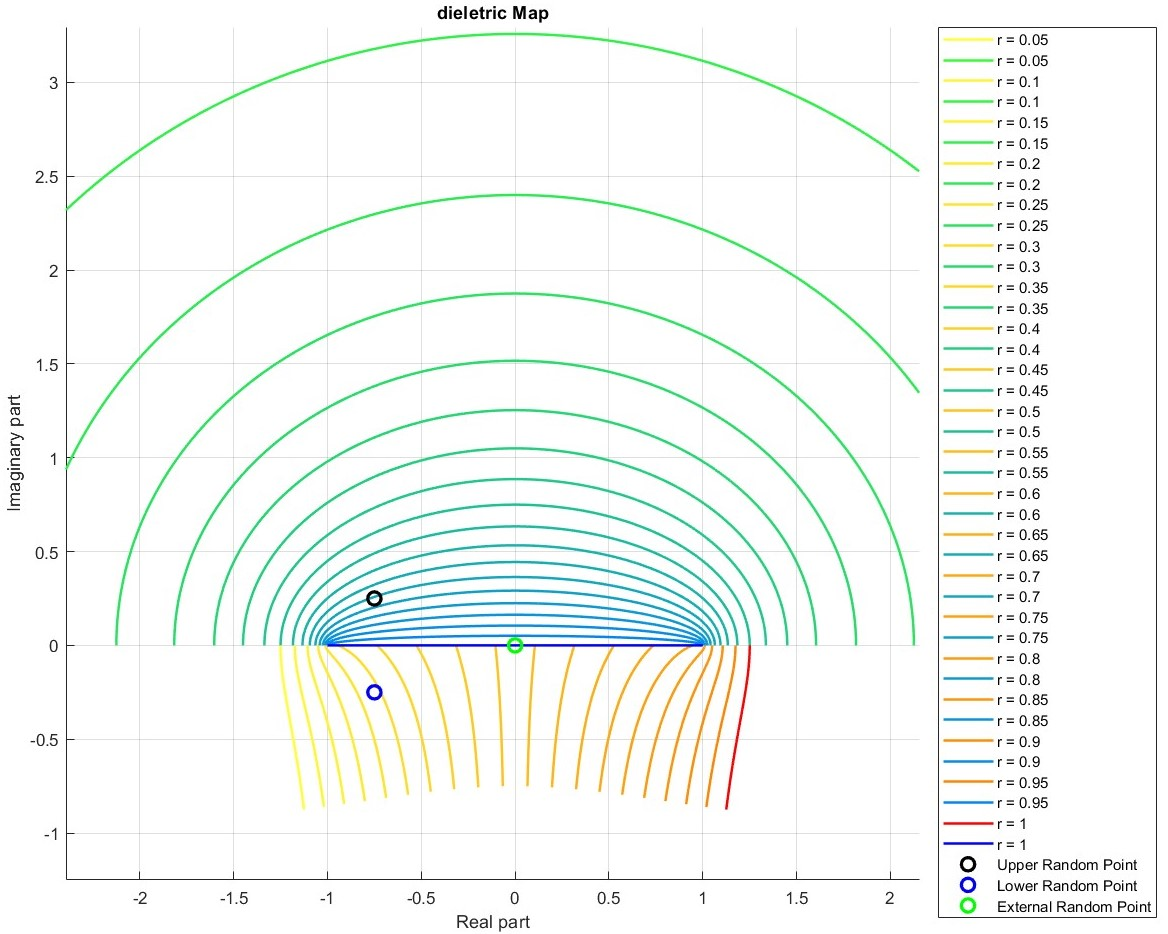
\includegraphics[width=0.5\linewidth]{Figs/map flat dieletric}} % Side by side images
    \caption{\small The point charge (the blue circle) and one of the induced charges (the black circle) in the disc. The left figure is the $\zeta$ plane, the right figure is the $z$ plane. The lower semi-circle (green and blue lines) map to the $y>0$ space, and the dielectric (yellow and red lines) map to $y<0$. The origin $\zeta=0$ maps to $\infty$, which fits the physical condition of the dielectric.\\
    Moreover, The dielectric area is compressed, and physically, $\epsilon$ may change, hence the dielectric is not linear anymore. This possible effect is ignored. 
}
    \label{fig:induce charge map}
\end{figure}

From the right figure of the $z$ plane, we see that the source charge (the blue circle) induced a charge (the black circle). For a point charge at $\zeta_{\alpha}=(-1-\im)$ in the dielectric, the corresponding induced charge inside the disc is at\vspace{-1.em}
\[\zeta_{o}=1/\zeta_{\alpha}=-\frac{1}{2}-\frac{1}{2}\im\vspace{-1.em}\]
and it maps to
\[
z_{o}=\frac{\zeta_{0}}{2}+\frac{1}{2 \zeta_{o}}=-\frac{3}{4}+\frac{1}{4}\im\]
Since the mapped dielectric is flat, take the conjugate to find $z_d=-\frac{3}{4}-\frac{1}{4}\im$, this is the location of the possibly twice-induced charge. The inverse map finds the twice-induced charge's location on the $\zeta$-plane is
\[
\zeta_d=z_d-\sqrt{z^2-1}=-1-\im
\]
This is where the source charge is located; hence, there will be no continuous charge generation.

The two induced charges in the complex equation are located within a conducting disc, where a real free charge cannot reside from a physics perspective. Therefore, they should represent an cumulative effect of the surface charges in the disc and induce no further charges.

\iffalse
This means the conformal mapping captures the physics property of the geometry of the dielectric. A further question is how the equipotential line requirement is fitted, as the dielectric area is rather ordinary. It will be discussed later.

The next question is, will the charge in the unit disc induce a charge in the dielectric? verified via conformal mapping, if it does, the location will be the location of the source charge. 


\begin{itemize}
    \item The induced charge of the source charge will not lie within the disc but will instead be projected onto the opposite side of the disc, and it generates a corresponding charge distribution within the conductive disc.
    \item The potential inside the dielectric is the superposition of the potentials generated by the source charge, its image charge, and the corresponding charge distribution within the disc.
    \item The potential outside the dielectric is equivalent to the potential generated by a smaller charge together with a conductive disc.
    \item The charges within the disc will not generate induced charges (either in the dielectric or elsewhere). There will be no free charges located inside the conductor, and this charge is a substitute for several induced surface charge distributions and therefore will not generate further induced charges.
\end{itemize}
Therefore, the internal voltage of the dielectric we proposed earlier is sufficient, with limited charge adjustment and compensation.

\fi

\subsection{The Potential on the $\zeta$-plane}\label{cpt:pot_zeta}
\hspace{0em}\indent The voltage has two parts, according to section (\ref{cpt:shield}). Assume the voltage in the air is the sum of a point charge (magnitude to be determined) and the induced charges in the disc. The complex potential of above is found to be\vspace{-1em}
\begin{equation}\label{eqn:w_up}
    w_{+}(\zeta) = \frac{q}{\pi \epsilon_0}\frac{1}{\epsilon_r+1} \im \left[ \log(\zeta - \zeta_0) - \log\left(\frac{1}{\zeta} - \overline{\zeta_0}\right) \right]\vspace{-1em}  
\end{equation}
\begin{figure}[H]
    \centering
    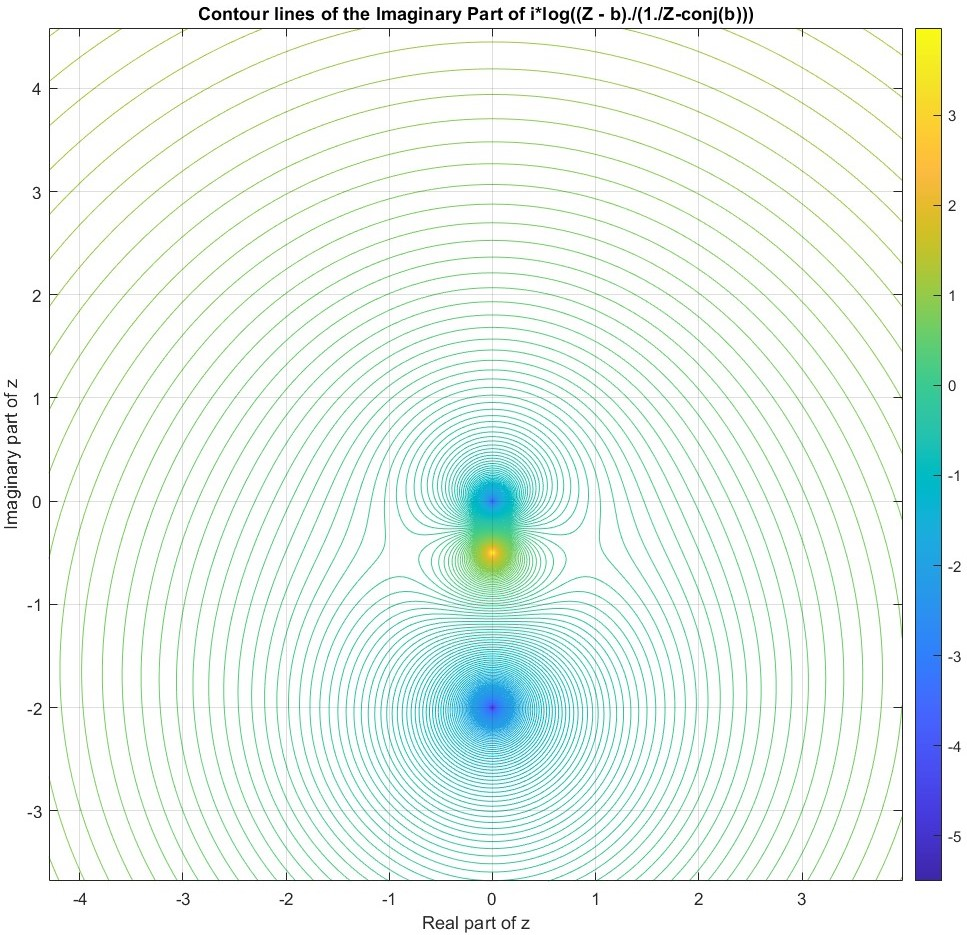
\includegraphics[width=1.\linewidth]{Figs/equal-pot, disk and charge, far view.jpg}
    \caption{\small The equipoentials from above. $y=0$ is the boundary between the dielectric and air. The three charges are the source charge at $(0, -2)$, and the two induced charge inside the disc. One at the origin, with the same sign of the source charge, and one differ. The equipoential of the disck is roughly visible.}
    \label{fig:enter-label}
\end{figure}

For the voltage below, start from charges (of different magintudes) in $W_+$, we need to determine the position and proportion the induced charge to meet the boundary conditions.

After some manipulation and trials, we derived that, the induced charge must be locate at $\overline{\zeta}_0$ above the disc. Previously, we found the structure with $q_t$ at $\overline{\zeta}_0$,  $q_b$, $q_r$ at ${\zeta}_0$ satisfies the conditions. Hence for the two charge at $\zeta_0$, and $1/\overline{\zeta_0}$, the corresponding charges must replicate the structure. Additionally, the charges at the origin do not affect surface charge distribution or the continuity of the voltage. 

\begin{figure}[H]
    \centering
    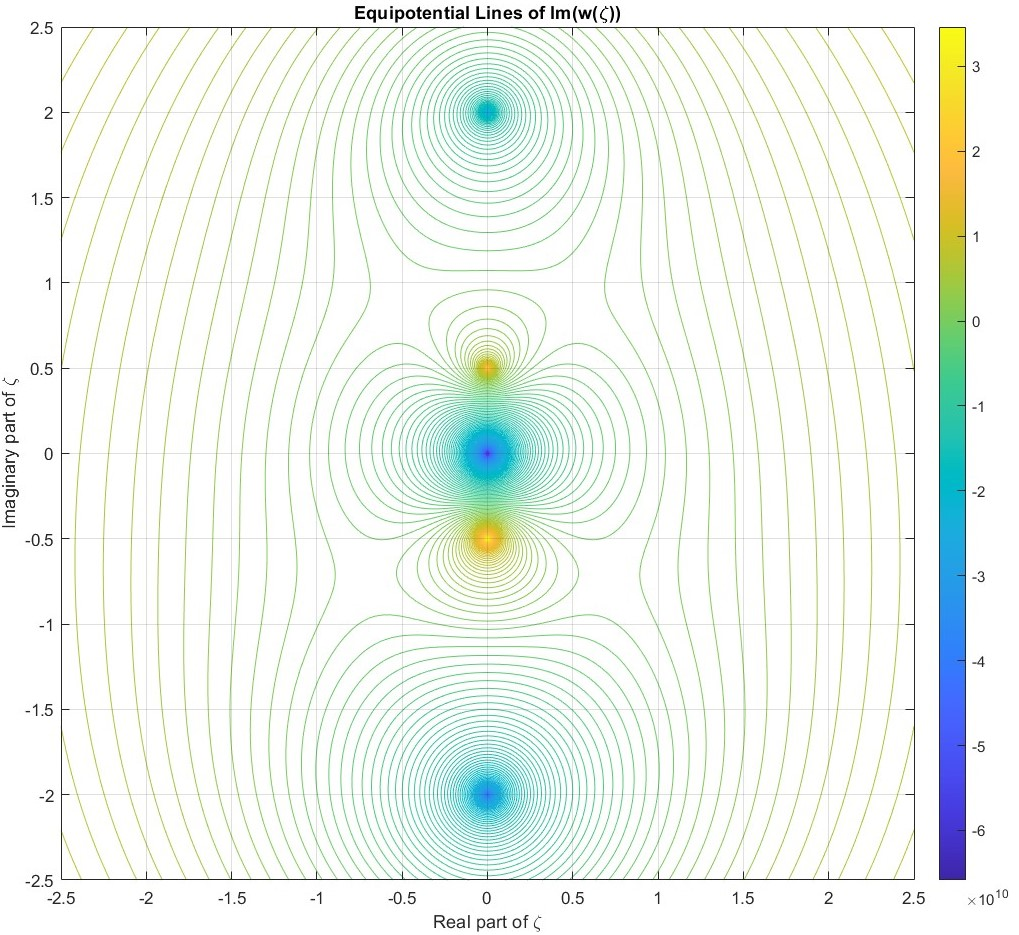
\includegraphics[width=1.\linewidth]{Figs/disc phase, inside dieletric.jpg}
    \caption{The equipotential from below. the potential contains six point charges, three of magnitude $q_b$ located separately at the source charge position, inside the semi-circle below, and the origin. Three of the fractions of the source charge $q_r$ are located symmetrically about the $y$-axis. Thus, there are two charges at the origin.}
    \label{fig:w_down}
\end{figure}


The complex potential of the dielectric area below $y=0$, of Figure (\ref{fig:w_down}) is \vspace{-.5em}
\begin{equation}\label{eqn:w_down}
    w_{-}(\zeta) = \frac{q}{2\pi \epsilon_0\epsilon_r} \im \left[ \log(\zeta - \zeta_0) - \log\left(\frac{1}{\zeta} - \overline{\zeta_0}\right) \right]
+\frac{q}{2\pi \epsilon_0\epsilon_r}\frac{\epsilon_r-1}{\epsilon_r+1}\im \left[ \log(\zeta - \overline{\zeta_0}) - \log\left(\frac{1}{\zeta} - \zeta_0\right) \right]    
\end{equation}
We check the voltage continuity at $y=0$, the other boundary conditions are satisfied simultaneously. From equation (\ref{eqn:w_up}) and equation (\ref{eqn:w_down}), \vspace{-1.em}
\[
V_+= \frac{q}{\pi \epsilon_0}\frac{1}{\epsilon_r+1} \left\{ \log\left(\sqrt{x^2+d^2}\right) -\log\left|\frac{1-\zeta\overline{\zeta_0}}{x}\right| \right\}
\]
\[
V_-= \frac{q}{2\pi \epsilon_0\epsilon_r} \left\{ \log\left(\sqrt{x^2+d^2}\right) -\log\left|\frac{1-\zeta\overline{\zeta_0}}{x}\right| \right\}
+\frac{q}{2\pi \epsilon_0\epsilon_r}\frac{\epsilon_r-1}{\epsilon_r+1} \left\{\log(\sqrt{x^2+d^2}) - \log\left|\frac{1-\zeta\zeta_0}{x}\right| \right\}
\]
We see that the three $\{...\}\coloneqq\alpha$ are equal on the $x-$axis, hence  \vspace{-1.em}
\[
V+=\frac{q}{\pi \epsilon_0}\frac{1}{\epsilon_r+1} \alpha\]
\[
V_-=\left(\frac{q}{2\pi \epsilon_0\epsilon_r} +\frac{q}{2\pi \epsilon_0\epsilon_r}\frac{\epsilon_r-1}{\epsilon_r+1}\right)\alpha
=\frac{q}{2\pi \epsilon_0\epsilon_r}\left( 1+\frac{\epsilon_r-1}{\epsilon_r+1}\right)\alpha
=\frac{q}{2\pi \epsilon_0\epsilon_r}\frac{2\epsilon_r}{\epsilon_r+1}\alpha=V_+
\]

\subsection{Mapping the Complex Potential to the $z$-plane}\label{cpt:slit_pot}
Next, we find a mapping $\zeta(z)$ from the semi-circle above to the slit, as Figure \ref{fig:map above} shows. The desired complex potential on the $z$-plane would be $w(\zeta(z))$.\vspace{-0.5em}
\begin{figure}[H]
    \centering
\adjustbox{frame=0.25pt,frame,margin=0.15,color=mycolor}{
    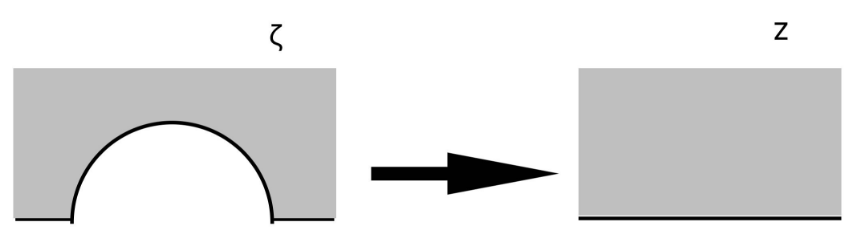
\includegraphics[width=1.\linewidth]{Figs/slit map brief.png}}
    \caption{\small The Mapping to addressing the charge, dielectric and slit problem. the shaded area represents the air and the upper arc of the disc, corresponding to the upper edge of the slit.}
    \label{fig:map above}
\end{figure}
\vspace{-0.5em}
In Matlab, $\zeta=z-\sqrt{z^2-1}
$ maps the left half of $\zeta$ plane, except the unit disc, to the left half of $z$ plane, and $\zeta=z+\sqrt{z^2-1}$ maps the right half of the $\zeta$ plane, except for the unit disc, to the right half of $z$ plane. Following the setting in Matlab, the complex potential on the $z$-plane is therefore divided into four parts.

Figure \ref{fig:vz above} is the equipotential of the voltage in the region $y>0$, on the $z$-plane\footnote{The $w(r<1)$ region must be excluded in the mapping. For an incorrect example see Appendix \ref{fig:wrong pot}.}. 

\begin{figure}[H]
    \centering
    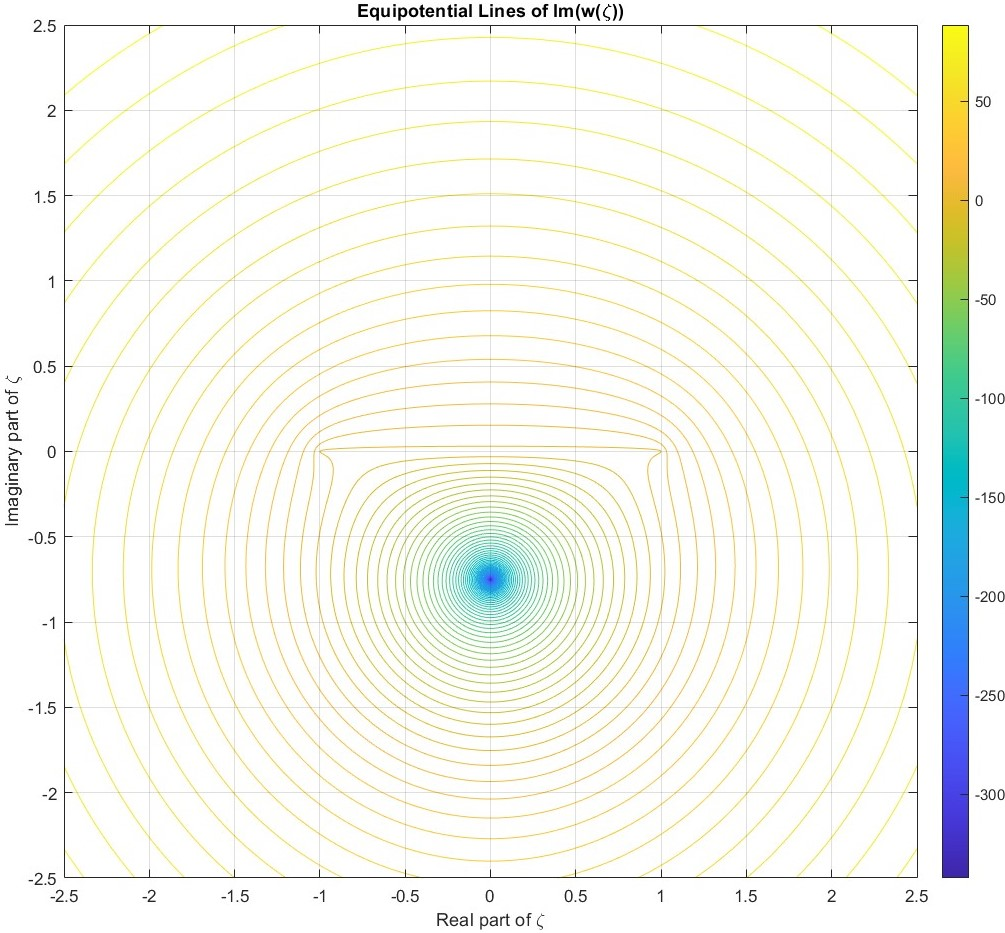
\includegraphics[width=1.\linewidth]{Figs/slit, Pot out dielectric, right.jpg}
    \caption{\small The equipotential lines of the area $y>0$, the 1, 2 quadrants. The dielectric is located in the region $y<0$. The slit is at $(x\in\pm1,y=0)$, and there is one equipotential intersect the slit. This is analogous  to streamline of a vortex under the slit of fluid dynamic. The source charge is at the centre of the concentric circles inside the dielectric.}
    \label{fig:vz above}
\end{figure}
For the complex potential above on the $z$-plane, start from equation (\ref{eqn:w_up}), leave $\zeta_0$ unchanged, use $\zeta(z)$ replacing $\zeta$ to rewrite $w(\zeta)$. In the first quadrant $(x>0, y>0)$, the complex potential is\vspace{-0.5em}
\[
\prescript{1}{}{w_{+}(z)} =\frac{q}{\pi\epsilon_0\epsilon_r}  \im \left[\log\left(z+\sqrt{z^2-1} - \zeta_0\right) - \log\left(\frac{1}{z+\sqrt{z^2-1}} - \overline{\zeta_0}\right)\right] \vspace{-0.5em}
\]
and in the second quadrant$(x<0, y>0)$, \vspace{-0.5em}
\[
\prescript{2}{}{w_{+}(z)} = \im \left[\log\left(z-\sqrt{z^2-1} - \zeta_0\right) - \log\left(\frac{1}{z-\sqrt{z^2-1}} - \overline{\zeta_0}\right)\right] \vspace{-2.em}
\]
    \begin{figure}[H]
        \centering
        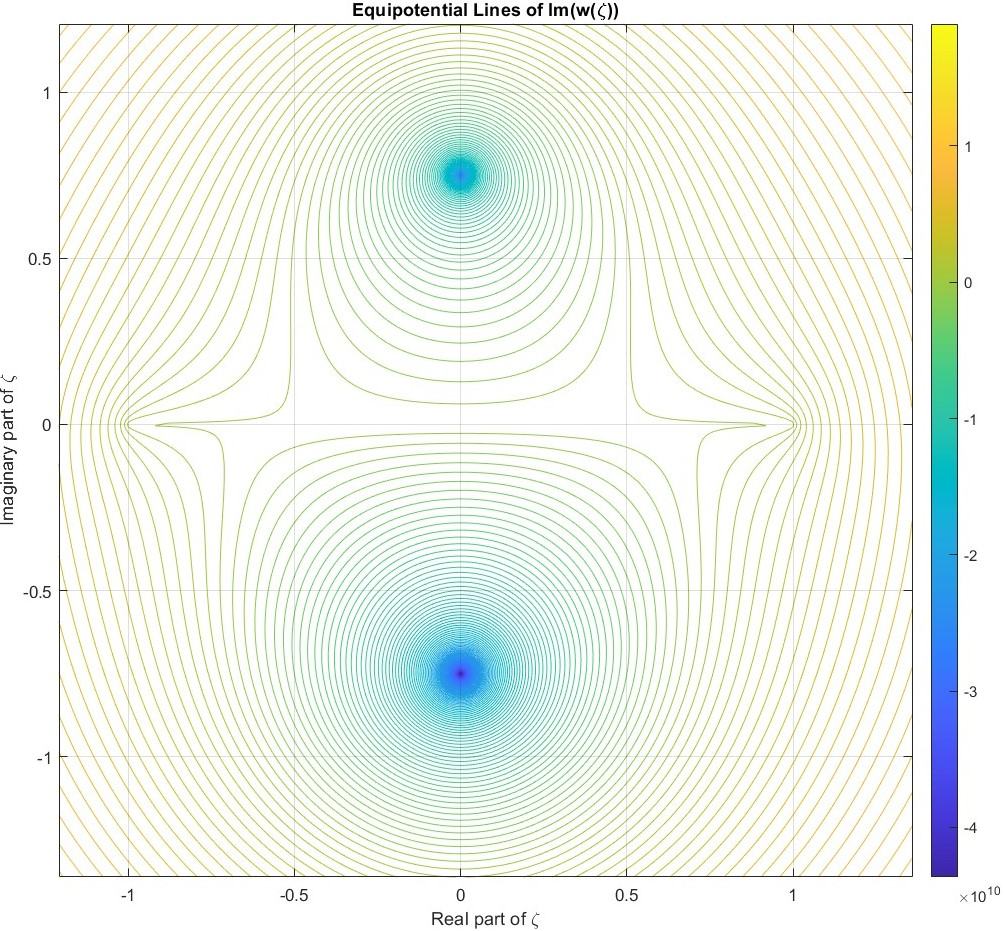
\includegraphics[width=1.\linewidth]{Figs/disc phase, inside dieletric, maped.jpg}
        \caption{\small The equipotentials in the region $y<0$, the 3, 4 quadrants. There is an induced charge above the dielectric. The slit is at $(x\in\pm1,y=0)$. One equipotential line reaches the slit, and the dense lines around the two cusps resemble the flow past a slit in fluid dynamics.}
        \label{fig:enter-label}
    \end{figure}\vspace{-1.em}
In the third quadrant$(x<0,y<0)$ and the fourth quadrant$(x>0,y<0)$, by equation (\ref{eqn:w_down}), we find the complex potentials are\vspace{-0.5em}:
\begin{align*}
\prescript{3}{}{w_{-}(z)} &= \frac{q}{2\pi \epsilon_0\epsilon_r} \im \left[ \log(z-\sqrt{z^2-1} - \zeta_0) - \log\left(\frac{1}{z-\sqrt{z^2-1}} - \overline{\zeta_0}\right) \right]\\
&+\frac{q}{2\pi \epsilon_0\epsilon_r}\frac{\epsilon_r-1}{\epsilon_r+1}\im \left[ \log(z-\sqrt{z^2-1} - \overline{\zeta_0}) - \log\left(\frac{1}{z-\sqrt{z^2-1}} - \zeta_0\right) \right]\vspace{-2.em}
\end{align*}
\begin{align*}
\prescript{4}{}{w_{-}(z)} &= \frac{q}{2\pi \epsilon_0\epsilon_r} \im \left[ \log(z+\sqrt{z^2-1} - \zeta_0) - \log\left(\frac{1}{z+\sqrt{z^2-1}} - \overline{\zeta_0}\right) \right]\\
&+\frac{q}{2\pi \epsilon_0\epsilon_r}\frac{\epsilon_r-1}{\epsilon_r+1}\im \left[ \log(z+\sqrt{z^2-1} - \overline{\zeta_0}) - \log\left(\frac{1}{z+\sqrt{z^2-1}} - \zeta_0\right) \right]\vspace{-0.5em}
\end{align*}
Combining the four parts we have the voltage across the entire $z$ plane, and the equipotentials.
    \begin{figure}[H]
        \centering
        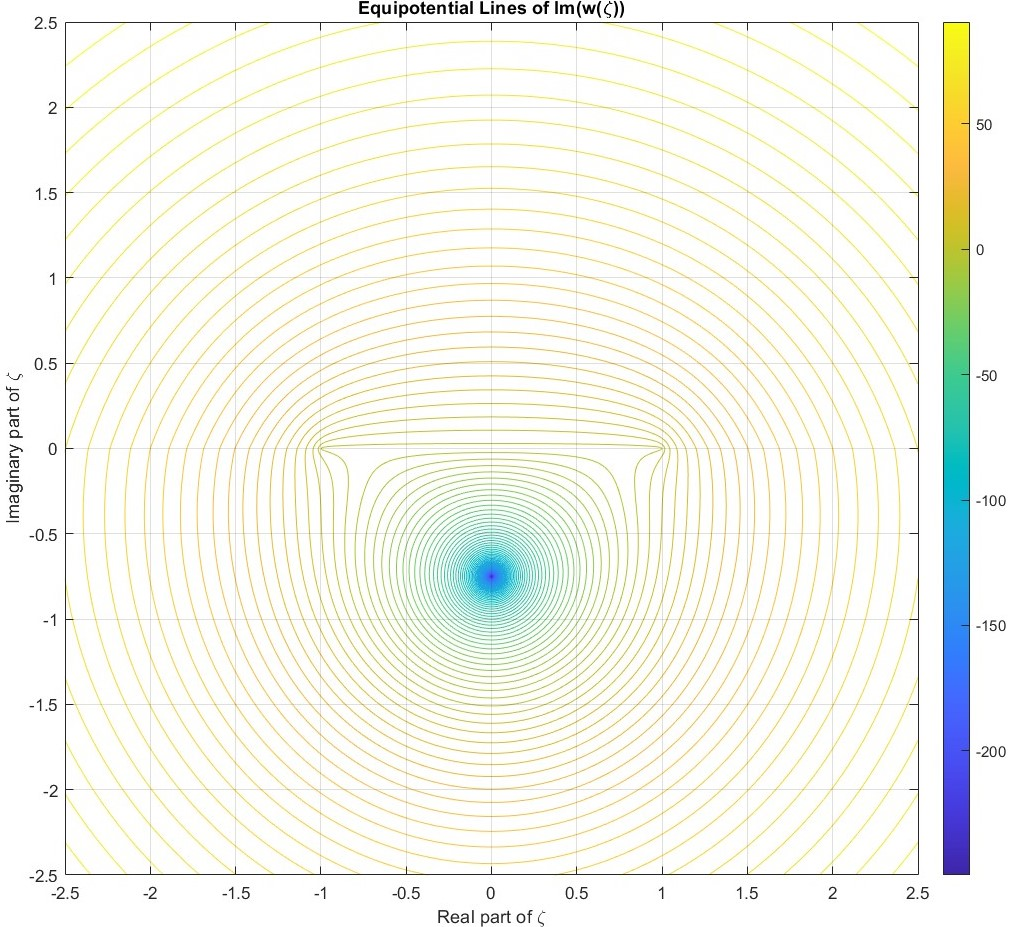
\includegraphics[width=1.\linewidth]{Figs/whole slit vot.jpg}
        \caption{\small The equipotentials of the entire plane are a combination of four parts. The slit is at $(\pm1,y=0)$. The induced charge is not seen. There is a slight distortion of voltages at $y=0$, the boundary between the dielectric and the region above.}
        \label{fig:enter-label}
    \end{figure}
 

